\subsection{Approval, Execution, and Evidence}
\label{sec:mech}
Approval depends on the operation route. For a single-node
\texttt{optimization\_explore} request in manual mode, the handler sends the
node, requested value, current effective interval, and rationale to the
approval service. It waits for a decision before calling the governed write
operation; a decline or timeout returns without reaching the controller, and
no dispatch occurs while the request is pending. Once approved, the handler
rechecks the node binding and applicable channel grant. The shared controller
then evaluates the current engineering, parameter, product, and recipe limits.
Outside benchmark mode, agent- or manual-source writes also face step,
interval, and hold-window checks before dispatch to the configured driver.
Unlike the recipe path described below, this single-node path does not use a
recipe-operation context snapshot. Revalidation does not establish an atomic
snapshot spanning the external device write.

Recipe operations follow a separate approval path. For \texttt{recipe\_trial}
and \texttt{recipe\_apply}, approval is bound to the operation and active
line--product--recipe--run context. After approval, the handler rechecks
authority and context, then verifies the recipe definition and candidate scope
before dispatch. A changed context, revoked binding, or changed recipe
definition prevents the proposal from proceeding. Recipe-trial approvals
remain valid for 30 minutes by default; single-node approval waits expire
after 180\,s. Outside benchmark mode, agent- and manual-source writes require
at least 60\,s between setpoint changes; recipe trials also use a default
per-line cadence of 300\,s.

Fig.~\ref{fig:hitl} contrasts the bounds used for online node writes in
Eq.~(\ref{eq:admission}) with those used for a replacement recipe, and shows
the route-dependent approval and shared-dispatch paths.

\begin{figure*}[t]
\centering
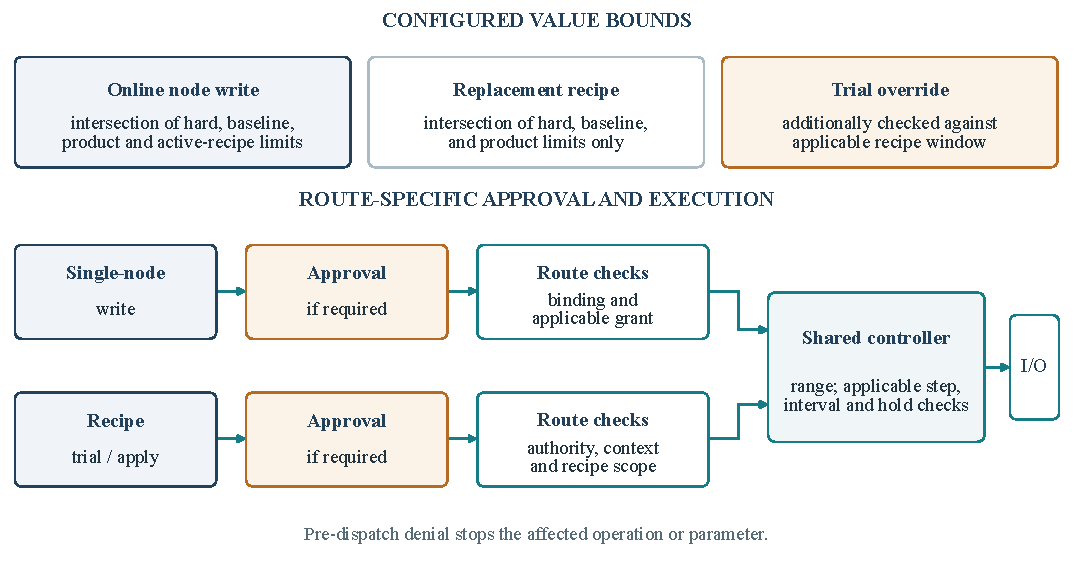
\includegraphics[width=\textwidth]{../figures/fig4.pdf}
\caption{Write admission and route-dependent approval. An online node write uses the intersection of hard, baseline, product, and active-recipe bounds; a replacement recipe is checked against hard, baseline, and product bounds, not the previous recipe window. Trial overrides are additionally checked against the applicable recipe window. After required approval, the routes recheck their applicable binding, grant, context, and recipe scope. The shared controller applies range checks; step, interval, and hold-window checks apply to agent or manual sources outside benchmark mode. A failed pre-dispatch check prevents the affected operation or parameter from reaching the driver.}
\label{fig:hitl}
\end{figure*}

A \texttt{recipe\_trial} illustrates this path. The handler checks the bound
recipe, active run, candidate parameters, and route timing. If approval is
required, it requests a decision and then revalidates authority and context
before submitting a bounded batch through the configured driver. It returns a
result for each parameter. Parameters are attempted individually, so a batch
can be partially applied; the per-parameter results and device state must be
reconciled before retrying. A trial does not save or apply a recipe version.
Callers can retrieve later DAQ observations separately before updating,
applying, or rolling back a recipe. The driver registry maps semantic controls
to configured protocol drivers, so operation arguments contain no
protocol-specific details.

Receipts record command outcomes; observations record subsequent process
behavior. Command results are graded as readback-verified,
transport-acknowledged, or unverified. A readback mismatch can trigger up to
three reads at 2\,s intervals, and recipe batches retain verification
outcomes for each parameter. A readback-verified result means that the
returned value matched the request. A transport acknowledgement alone does not
establish that the device applied the value, and an unverified result does not
establish a matching readback. DAQ stores later timestamped process
observations; recipe history, approvals, and task records remain with
their owning services. Identifiers and timestamps can link these records
when available, but a later observation alone does not prove that the command
caused the measured change. Section~\ref{sec:eval} evaluates selected parts
of this evidence chain under the stated test conditions.

